\section{General Model Implementation}

% Problem, context, solution

Models are contructed from agents that have functions. These functions must be
executed in a correct order for the model to run correctly. Formerly this order
was defined in the model definition XMML by dependencies between functions. These
dependencies could be either internal, within individual agents, or
communication, dependent on messages from other agents. This was enough
information to be able to order functions and plan communication sychronisation
points to work in parallel.

The economic models eventually started to run only certain functions at
certain times, for example, weekly or monthly. Because each function
was still being executed this required a condition at the start of every
function and soon became a hinderance. Even though a series of functions used
the same time series they all had to include the same condition. This was also
true of other conditions, for example only households that were unemployed need
execute functions involved with the labour market.

This was solved by defining the model in the XMML as a state machine. Where
states are defined before and after functions.
Each state can have many incoming functions and many outgoing functions.
Only the unique start state has no incoming functions, and end states have no
outgoing functions. This then allows branches of functions where the condition
for all the functions can be defined at the start of the branch.

This can be shown by Figures \ref{fig:depends} and \ref{fig:state}.

\begin{figure}[hb]
\begin{minipage}[b]{0.5\linewidth}
\centering
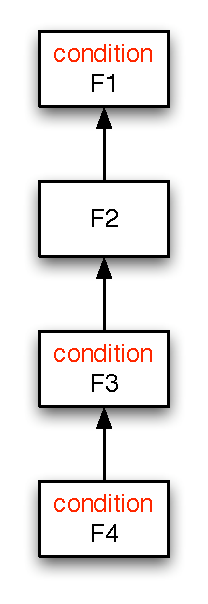
\includegraphics[scale=0.5]{depends_graph.eps}
\caption{Dependency graph model}
\label{fig:depends}
\end{minipage}
\hspace{0.5cm}
\begin{minipage}[b]{0.5\linewidth}
\centering
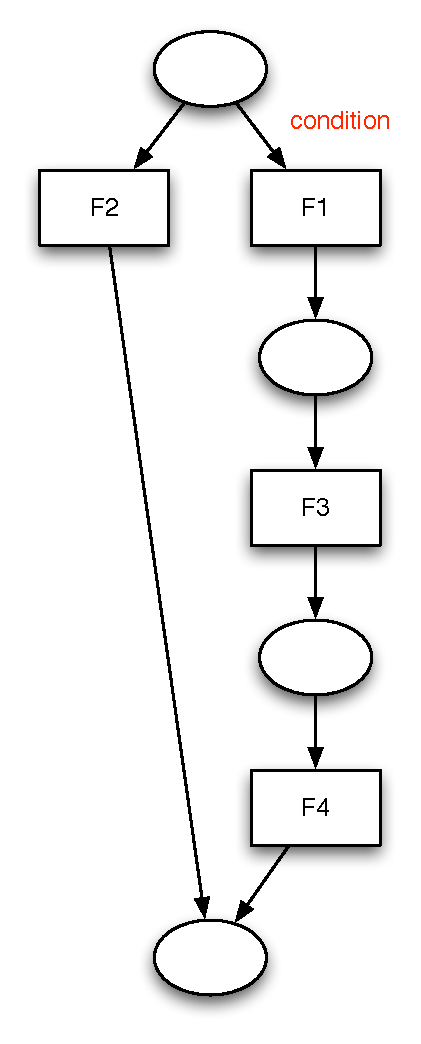
\includegraphics[scale=0.5]{state_graph.eps}
\caption{State graph model}
\label{fig:state}
\end{minipage}
\end{figure}

The model can now be recognised as a state machine but with the restriction
that once a state has been entered by an agent it cannot reenter the same
state. This provides sychronisation of agents in parallel during execution. Also
input to functions are sets of inputs (messages) which can be empty. This is
the level of detail required by FLAME to plan the communication sychronisation
in parallel.

Each function can then be defined by the parameters as shown in Table
\ref{tab:funcparameters}, where $M_{pre}$ is the pre-condition of the memory
and $M_{post}$ is the post-condition of the memory.

\begin{table}[hbp]
\centering
\begin{tabular}{|l|l|l||l||l|l|l|}
\hline
Current State&Input&$M_{pre}$&Function&$M_{post}$&Output&Next State\\
\hline
\end{tabular}
\caption{Function parameters} \label{tab:funcparameters}
\end{table}

In XMML this is currenly written as below where $M_{pre}$ is defined as
\textit{condition} and $M_{post}$ is written as source code within a function
with the same name as the function name.

\begin{mylisting}
\begin{verbatim}
<function>
 <name>Function_name</name>
 <description>A description of the function</description>
 <currentState>current_state</currentState>
 <nextState>next_state</nextState>
 <condition>condition</condition>
 <inputs>inputs</inputs>
 <outputs>outputs</outputs>
</function>
\end{verbatim}
\end{mylisting}

